\documentclass{standalone}
\usepackage{../../../../preamble_formulas}
\begin{document}
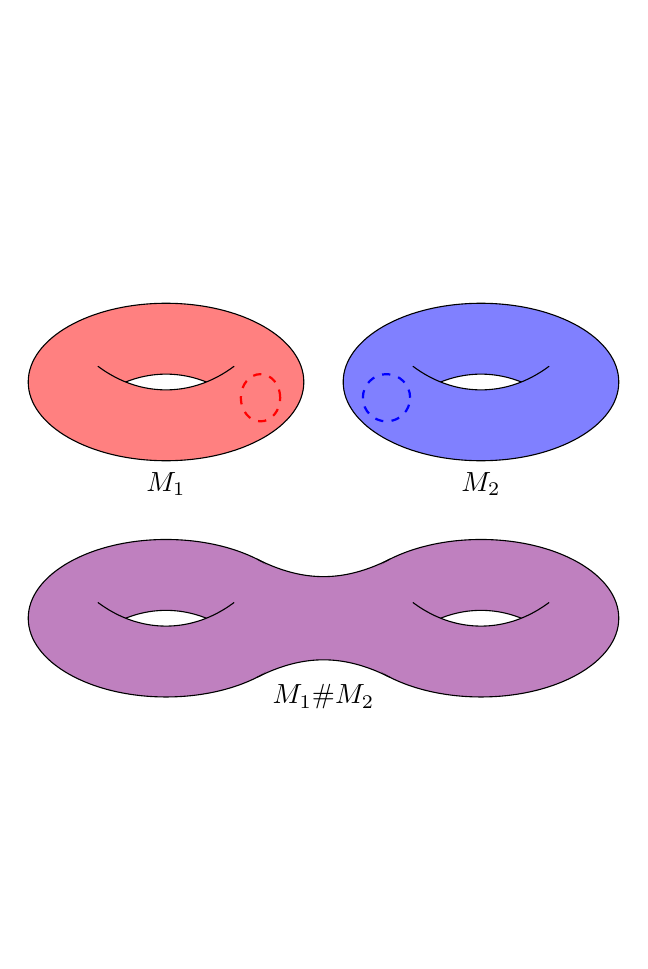
\begin{tikzpicture}
  \def\a{2}
  \def\b{0.5}
  \def\manifold#1#2#3#4{
    % \draw plot [smooth cycle,tension=0.8] coordinates{(-0.1+#1,0+#2) (-\a+#1,-2*\b+#2) (-2*\a+0.5+#1,0+#2) (-\a+#1,2*\b+#2)};
    % \filldraw[draw=black,fill=#4] (-\a+#1,#2) ellipse (1.75 and 1);
    % % hole
    % \draw[name path=A] plot [smooth,tension=0.75] coordinates{(-\a+0.75+#1,0.2-0.15+#2) (-\a+#1,0-0.15+#2) (-\a-0.75+#1,0.2-0.15+#2)};
    % \draw[name path=B] plot [smooth,tension=0.75] coordinates{(-\a+0.5+#1,-0.2+0.15+#2) (-\a+#1,0+0.15+#2) (-\a-0.5+#1,-0.2+0.15+#2)};
    % \tikzfillbetween[of=A and B]{white};
    % \node at (-\a+#1,-1.3+#2){#3};
    \draw[fill=#4] (#1,#2) ellipse (1.75 and 1);
    \begin{scope}
      \clip (#1,#2+2.2) ellipse (1.75 and 2.3);
      \draw[fill=white] (#1,#2-2.2) ellipse (1.75 and 2.3);
    \end{scope}
    \begin{scope}
      \clip (#1,#2-1.8) ellipse (1.75 and 2.3);
      \draw (#1,#2+2.2) ellipse (1.75 and 2.3);
    \end{scope}
    \node at (#1,-1.3+#2){#3};
  }

  %%% M1
  \manifold{-\a}{3}{$M_1$}{red!50}
  \draw[red,dashed, thick] (-\a/2+0.2,3-0.2) ellipse (0.25 and 0.3);

  %  %%% M2
  \manifold{\a}{3}{$M_2$}{blue!50}
  \draw[blue,dashed, thick] (\a/2-0.2,3-0.2) circle (0.3);


  %%% M1+M2
  \manifold{-\a}{0}{}{red!50!blue!50}
  %  \draw[red,dashed, thick] (-\a/2+0.2,3-0.2) ellipse (0.25 and 0.3);

  \manifold{\a}{0}{}{blue!50!red!50}
  %  \draw[blue,dashed, thick] (\a/2-0.2,3-0.2) circle (0.3);

  % \draw plot [smooth cycle,tension=0.8] coordinates{(0,\b) (\a,2*\b) (2*\a-0.5,0) (\a,-2*\b) (0,-\b) (-\a,-2*\b) (-2*\a+0.5,0) (-\a,2*\b)};

  % % right hole
  % \draw plot [smooth,tension=0.75] coordinates{(\a-0.75-0.15,0.2-0.15) (\a-0.15,0-0.15) (\a+0.75-0.15,0.2-0.15)};
  % \draw plot [smooth,tension=0.75] coordinates{(\a-0.5-0.15,-0.2+0.15) (\a-0.15,0+0.15) (\a+0.5-0.15,-0.2+0.15)};

  % % left hole
  % \draw plot [smooth,tension=0.75] coordinates{(-\a+0.75+0.15,0.2-0.15) (-\a+0.15,0-0.15) (-\a-0.75+0.15,0.2-0.15)};
  % \draw plot [smooth,tension=0.75] coordinates{(-\a+0.5+0.15,-0.2+0.15) (-\a+0.15,0+0.15) (-\a-0.5+0.15,-0.2+0.15)};
  \node at (0,-1){$M_1\#M_2$};

  % \draw[red!50]
  % (-0.469,-0.484) to[out=49.924,in=-49.924]
  % (-0.469,0.484);
  % \draw[blue!50]
  % (0.469,0.484) to[out=180+49.924,in=180-49.924]
  % (0.469,-0.484);

  \fill[blue!50!red!50]
  (-0.8425,0.75) to[out=-26.746,in=180+26.746]
  (0.8425,0.75) to[out=180+26.746,in=180-26.746]
  (0.8425,-0.75) to[out=180-26.746,in=26.746]
  (-0.8425,-0.75) to[out=26.746,in=-26.746]
  (-0.8425,0.75);
  \draw[black]
  (-0.8425,0.75) to[out=-26.746,in=180+26.746]
  (0.8425,0.75)
  (0.8425,-0.75) to[out=180-26.746,in=26.746]
  (-0.8425,-0.75);
\end{tikzpicture}

\end{document}